\subsection{Problema a resolver}

El siguiente ejercicio se da en el contexto de un museo donde se requiere, por cuestiones de seguridad, colocar sensores de forma tal que todo el piso esté cubierto por los lásers que estos emiten. Existen dos tipos de sensores: los bidireccionales (que emiten señales horizontales o verticales) y los cuatridireccionales (que emiten señales verticales y horizontales). Los precios de éstos son \$4000 y \$6000 respectivamente. Se pide, también, que un sensor no apunte hacia otro dado que esto podría dejarlos sin funcionar. Además, se pide que ciertos lugares, definidos como \textit{importantes}, sean atravesados por dos lásers simultáneamente. El objetivo del algoritmo a realizar consiste en encontrar una forma de colocar los sensores de manera que el suelo quede completamente cubierto y que los lugares \textit{importantes} estén atravesados por un láser horizontal y otro vertical utilizando el mínimo costo posible. Por otra parte, debe ser tenido en cuenta que el museo cuenta con paredes que pueden interferir los lásers de los sensores.\newline

\newline
\textbf {Formatos de entrada y salida:}\newline
\newline
La entrada del algoritmo contiene una instancia del problema. La primera línea indica las dimensiones $n$ y $m$ de la grilla. A esta línea le siguen $n$ líneas, cada una con $m$ valores separados por espacios, indicando el contenido de cada una de las $n$ x $m$ casillas de la grilla, donde un 0 representa una pared, un 1 representa un casillero libre común y un 2 representa un casillero libre importante.\newline

En el caso en el que el problema no tenga solución, la salida deberá contener únicamente una línea con el valor -1. Caso contrario, la salida debe comenzar con dos números enteros: 
$$S\ C$$ 
donde $S$ es la cantidad de sensores utilizados y $C$ es el costo toal de la solución. Luego, para cada sensor utilizado, debe haber una línea con el siguiente formato: 
$$t\ f\ c$$ 
donde $t$ es el tipo de sensor y $(f,c)$ son la fila y columna en donde éste se ubica (la esquina superior izquierda de la grilla es la posición (1,1) y la inferior derecha es la $(n,m)$). Para los sensores cuatridireccionales, $t$ debe valer 1, para los bidireccionales en forma horizontal $t$ debe valer 2 y en forma vertical 3.\newline
\newline
Un ejemplo de este problema es el que está provisto por la cátedra:

\begin{figure}[H]
	\begin{center}
		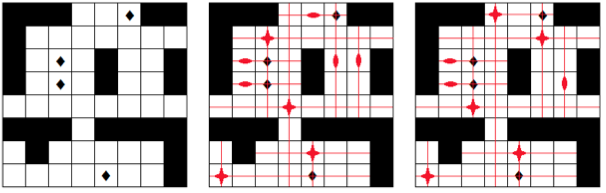
\includegraphics[width=320pt]{../imgs/ej3_ejemploCatedra.png}
	\end{center}
\caption{Un ejemplo y dos soluciones distintas.}
\end{figure}

En el ejemplo de la Figura 1 el museo se ve representado por una cuadricula donde donde los cuadrados blancos representan el suelo, los cuadrados negros representan las paredes y los cuadrados que tienen un rombo dentro representan los lugares importantes, a continuación de la imagen se muestran dos posibles soluciones al problema, en las cuales las cruces rojas representan los sensores bidireccionales, y las lineas rojas gruesas representan los sensores horizontales y verticales, desde estos se extienden lineas rojas que representan el área que cubren estos sensores con lasers.

En el primer caso el costo total es de \$44000 y la segunda solución tiene un costo de \$42000.

\subsection{Resolución coloquial}

Para resolver el problema presentado decidimos utilizar la técnica de $backtracking$. Ésta consiste en evaluar las posibles combinaciones de soluciones del problema almacenándolas hasta llegar a la deseada. Para ello, definimos criterios de parada que nos permitieran decidir si las soluciones parcialmente obtenidas eran candidatas a soluciones válidas.\newline
\newline
Para lograr una correcta visualización del problema, representamos el piso entero del museo con una matriz, respetando las paredes y las casillas importantes. Luego, cada elemento de la matriz representa a una baldosa/casillero del piso y almacena el estado de la misma. Esto significa que de acuerdo a si contiene un 0, un 1 o un 2, podemos saber si hay algún sensor en ella o si le pasa algún láser por encima.\newline
\newline
Nuestro algoritmo, en primera instancia, genera un árbol de decisiones sobre todas las combinaciones posibles de cada casillero. Para lograrlo, recorre paulatinamente la matriz mencionada y, en cada paso, toma una decisión sobre el casillero actual para avanzar, luego, al siguiente. Las posibles decisiones son colocar o no algún sensor, empezando por intentar con el sensor cuatridireccional, para proseguir con el horizontal, luego el vertical y por último sin ningún sensor. Con el fin de acotar el tiempo de ejecución del algoritmo, se idearon ciertas cotas que frenan la ramificación del nodo que llega a algún caso que no tiene solución. Las cotas implementadas fueron las siguientes:
\begin{enumerate}
\item Una vez que se encuentra una solución, se almacena su costo y cualquier rama cuyo costo actual sea mayor al $almacenado-2000$ (siendo 2000 = diferencia entre un sensor cuatridireccional y uno bidireccional) es descartado.
\item Sobre las casillas importantes no puede haber ningún sensor cuatridireccional. Esto se debe a que en dicho caso, no existiría la posibilidad de atravesarlo por dos lásers sin que se rompan.
\item No puede haber ningún sensor vertical en las filas que tengan algún casillero importante, lo mismo para sensores horizontales en la columna. Esto se debe al mismo motivo mencionado en el ítem anterior.
\item Cualquier fila conteniendo algún sensor vertical no puede tener ninguno horizontal pues provocará un choque entre ellos. Análogamente de para una columna conteniendo un sensor horizontal a la que se le quiera agregar uno vertical.
\end{enumerate}
De este modo, el árbol realizado contiene en cada nodo una posibilidad de casillero y, como máximo, tres hermanos con las otras posibilidades. Luego, el árbol es recorrido y se comparan los precios de cada solución válida hasta llegar a una mínima.\newline
\newline

El pseudocódigo que describe la solución a nuestro problema es el siguiente:

\begin{algorithm}[H]
	\SetAlgoLined
	\caption{Algoritmo de Backtracking}
	\KwIn{Matriz $grilla$}
	\KwOut{Lista sensores}
	
	Matriz $mejorGrilla$
	Lista $casillasLibres$\\

	\For{Posicion $p \in grilla$}{
		\If{p esta libre}{
			$casillasLibres \leftarrow p$\\
		}
		\If{$p$ es importante}{
			\textbf{RestringirPorImportantes}(p)\\
		}
	}

	sensores := backtrack($grilla$, $casillasLibres$, $mejorGrilla$)\\

	\textbf{devolver} sensores
\end{algorithm}

\begin{algorithm}[H]
	\SetAlgoLined
	\caption{backtrack}
	\KwIn{Matriz $grilla$, Lista $casillasLibres$, Matriz $mejorGrilla$}
	\KwOut{Lista sensores}

    \If{$costoActual$ > $(mejorCostoObtenido - 2000)$}{
        backtrack($grilla$, $casillasLibres$)\\
	}
	
	\If{sensores esta vacio}{
		\If{chequearSolucion($grilla$) \land $ (costoActual $ < $ mejorCostoObtenido)$}{
			$mejorCostoObtenido$ := $costoActual$\\
			$mejorGrilla$ := $grilla$
		}
    }

	Casilla $casillaActual$ := Proxima casilla libre \in casillasLibres\\
	
	\If{$¬$sePuedeColocarUnSensor($casillaActual$)}{
		$mejorCostoObtenido$ := $costoActual$\\
		$mejorGrilla$ := $grilla$
	}
	
	\If{Puedo poner un sensor bidireccional en $casillaActual$}{
		Restringir por láser bidireccional\\
		Saco casillaActual de casillasLibres\\
		backtrack($grilla$, $casillasLibres$)\\
	}
	\If{Puedo poner un sensor vertical en $casillaActual$}{
		Restringir por láser vertical\\
		Restringir casilleros horizontales\\
		Saco casillaActual de casillasLibres\\
		backtrack($grilla$, $casillasLibres$)\\
	}
	\If{Puedo poner un sensor horizontal en $casillaActual$}{
		Restringir por láser horizontal\\
		Restringir casilleros verticales\\
		Saco casillaActual de casillasLibres\\
		backtrack($grilla$, $casillasLibres$)\\
	}

	Dejo el casillero en blanco\\
	backtrack($grilla$, $casillasLibres$)\\

	\textbf{devolver} ContarSensores($grilla$)
\end{algorithm}

\subsection{Demostración de correctitud}

Para demostrar la correctitud de nuestro algoritmo, debemos probar que se cumplen las siguientes propiedades:
\begin{itemize}
\item Nuestro algoritmo genera todas las combinaciones posibles para cada casillero.
\item Las podas utilizadas no alteran la solución final.
\item La solucion es óptima, es decir, no existe otra cuyo costo sea menor.
\end{itemize}

\newline

\textbf{Nuestro algoritmo genera todas las combinaciones posibles para cada casillero.} \newline

Esto lo realiza tomando el primer elemento (ignorando el anterior) e intentando ubicar algún sensor, o ninguno, siempre que este no se encuentre contemplado en las podas o que no rompa los casos especificados
 por el enunciado. Como resultado, por cada elemento, puede generar 4 casos posibles: 
 \begin{itemize}
 \item $sin$ $sensor$
 \item con $sensor$ $bidireccional$ $horizontal$  
 \item con $sensor$ $bidireccional$ $vertical$  
 \item con $sensor$ $cuatridireccional$ 
 \end{itemize}
  Asi sucesivamente con cada cuadricula, logrando asi, generar todas las permutaciones factibles. 

\textbf{Las podas utilizadas no alteran la solución final} \newline

Las podas utilizadas son:
\begin{itemize}
\item Poda sobre el costo : Sea T el costo de la mejor solucion generada por el algoritmo en determinado momento. Si cualquier otra solucion parcial ya alcaza el costo T-2000 pueden pasar dos cosas, o que el costo final sea T-2000 
o que el costo final sea mayor a T $($ya que menos es imposible dado que la diferencia que existe entre los sensores de de 2000 $)$. Luego nuestro algoritmo descarta aquellas soluciones parciales cuyos costos superen los T-2000
asegurando no eliminar soluciones factibles.  
\item Poda sobre casilleros importantes: Esta es trivial, ya que cualquier solucion que un casillero importante contenga un sensor cuatridimencional no va a permitir que ningun otro laser impacte sobre ese casillero.
\item Poda sobre mismas lineas: Esta tambien es trivial, ya que en la misma linea donde tengo un sensor bidireccional vertical no puedo poner una vertical, lo mismo para el sensor bidireccional horizontal. Y donde 
tengo un sensor cuatridimencional, no puedo poner ningun otro sensor en la misma linea.
\item Poda sobre lineas de casilleros importantes: Dado un casillero importante hay que asegurarse que dos lineas atraviesen al mismo, y como solo hay lineas horizontales y verticales, no puede haber soluciones
ddonde haya sensores bidireccionales verticales en los costados (misma linea horizontal) de un casillero importante; y no puede haber sensores verticales arriba o abajo (misma linea vertical) del casillero importante.
 Por lo tanto, esto no solo es una poda, sino una condicion necesaria de la solucion.
\end{itemize}

\textbf{La solucion es optima, es decir, no existe otra cuyo costo sea menor} \newline

Este se puede observar facilmente, ya que nuestro algoritmo a medida que va generando soluciones, ya guardando aquellas que tienen menor costo. De esta manera, el resultado final es la solucion con menor costo entre todas
las posibles.


\subsection{Complejidad del algoritmo}


Veamos paso a paso la complejidad del algoritmo de backtracking:

En la linea 1 se obtienen las posiciones libres de la grilla, esto se obtiene recorriendo secuencialmente todas las posiciones de la matriz y en cada paso pregunta si es una casilla libre o no, esta pregunta se hace en tiempo constante y recorrer todos los elementos tiene una complejidad de O($n*m$).

\subsection{Código fuente}


\subsection{Instancias posibles}
Para verificar la correctitud de nuestro programa, dispusimos variar estratégicamente las instancias de entrada al ejecutarlo.
\begin{itemize}
\item En primer lugar, ejecutamos el programa ingresando una única casilla libre, siendo ésta un lugar importante. Dicha prueba se realizó con el fin de verificar que nuestro algoritmo devolviera $-1$ dado que no existe la posibilidad de insertar 2 lásers en ese espacio, siendo este el requisito para los espacios importantes.\newline

\textbf{Parámetro de entrada:} 
$$3\ \ 3$$
$$0\ \ 0\ \ 0$$
$$0\ \ 2\ \ 0$$
$$0\ \ 0\ \ 0$$
\textbf{Parámetro de salida:} $$-1$$\newline
\item Por otra parte, probamos el programa para un museo conformado únicamente por paredes, en otras palabras, el caso vacío. Lo relevante de este caso es que nuestro algoritmo lo considera y otorga, como salida, que la solución es no colocar ningún láser.\newline




\textbf{Parámetro de entrada:} 
$$3\ \ 3$$
$$0\ \ 0\ \ 0$$
$$0\ \ 0\ \ 0$$
$$0\ \ 0\ \ 0$$
\textbf{Parámetro de salida:} $$0\ \ 0$$\newline
\item Otro caso interesante es analizar la solución obtenida al tener todos espacios libres. La idea de dicho caso consiste en comprobar que el algoritmo devuelve la solución más económica del problema.\newline

\textbf{Parámetro de entrada:} 
$$3\ \ 3$$
$$1\ \ 1\ \ 1$$
$$1\ \ 1\ \ 1$$
$$1\ \ 1\ \ 1$$
\textbf{Parámetro de salida:} 
$$3\ \ 12000$$
$$2\ \ 0\ \ 0$$
$$2\ \ 1\ \ 2$$
$$2\ \ 2\ \ 0$$
\newline

\item Por otra parte, resulta importante corroborar la solución en el caso en el que todos los espacios son importantes. En este caso particular no existe solución ya que no podrían pasar dos lásers por el mismo casillero especial sin que uno de estos toque a otro láser.\newline

\textbf{Parámetro de entrada:} 
$$3\ \ 3$$
$$2\ \ 2\ \ 2$$
$$2\ \ 2\ \ 2$$
$$2\ \ 2\ \ 2$$
\textbf{Parámetro de salida:} $$-1$$\newline

\item Otra situación posible es en la que se encuentran alternados los casilleros de piso y pared. De este caso puede destacarse que no es posible aplicar ninguna de las podas mencionadas.\newline
\textbf{Parámetro de entrada:} 
$$3\ \ 3$$
$$1\ \ 0\ \ 1$$
$$0\ \ 1\ \ 0$$
$$1\ \ 0\ \ 1$$
\textbf{Parámetro de salida:} 
$$5\ \ 20000$$
$$2\ \ 0\ \ 0$$
$$2\ \ 0\ \ 2$$
$$2\ \ 1\ \ 1$$
$$2\ \ 2\ \ 0$$
$$2\ \ 2\ \ 2$$

\begin{figure}[H] % indico que voy a poner una figura y [h] indica que la posición relativa, tambien puedo usar t = top entre otros.
\hfill
\begin{minipage}[t]{.45\textwidth}
\begin{center}
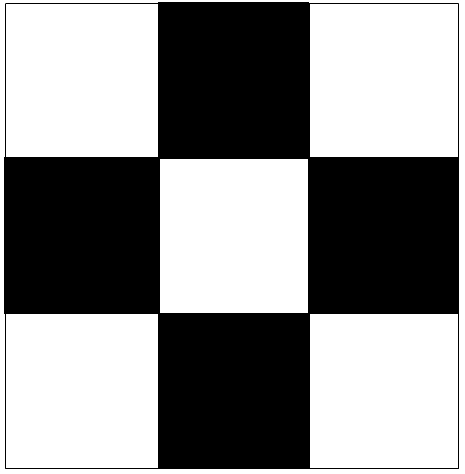
\epsfig{file=instanciaposible_ej3_in5.jpg, scale=0.15} % primera imagen colocada a la izquierda
\caption{Entrada de la instancia posible Nº1.}
\label{fig-tc1}
\end{center}
\end{minipage}
\hfill
\begin{minipage}[t]{.45\textwidth}
\begin{center}
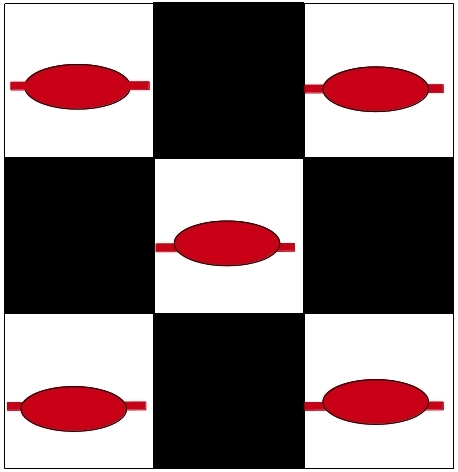
\epsfig{file=instanciaposible_ej3_out5.jpg, scale=0.15} % segunda imagen colocada a la derecha
\caption{Salida de la instancia posible Nº1.}
\label{fig-tc2}
\end{center}
\end{minipage}
\hfill
\end{figure}

\item Por último, se encuentra el caso en el que coexisten los 3 tipos de casilleros, siendo éste el mas típico del problema. \newline

\textbf{Parámetro de entrada:} 
$$3\ \ 3$$
$$1\ \ 1\ \ 1$$
$$1\ \ 2\ \ 0$$
$$0\ \ 0\ \ 1$$
\textbf{Parámetro de salida:} 
$$3\ \ 14000$$
$$1\ \ 0\ \ 1$$
$$2\ \ 1\ \ 0$$
$$2\ \ 2\ \ 2$$
\newline
\end{itemize}

\subsection{Testing}
Para realizar las pruebas de complejidad, generamos instancias aleatorias de pesos de cajas alterando la cantidad de las mismas pero manteniendo estático el peso máximo de carga de los camiones en 120 \unit{kg}. Estas instancias fueron generadas en $C++$ con la función $rand()$ de forma tal a poder acotarlas por la capacidad de carga de los camiones. La cantidad de cajas generadas se comprendió entre 5000 y 100000, agregando de a 5000 en cada iteración. De este modo, logramos medir las pruebas de nuestro algoritmo para comprobar que la complejidad correspondiera con la mencionada anteriormente.

